\chapter{Introduzione alla fisica delle particelle e il mesone $D^{*+}$ }

\section{Il Modello Standard}
Per quanto riguarda la fisica delle particelle, il modello che attualmente ne descrive i fondamenti è il \textit{Modello Standard}. In questo modello le particelle fondamentali sono divise tra fermioni e bosoni. La \ref{fig:ModelloStandard} rappresenta uno schema delle particelle previste dal Modello Standard.

    \begin{figure}[htbp]
        \centering
        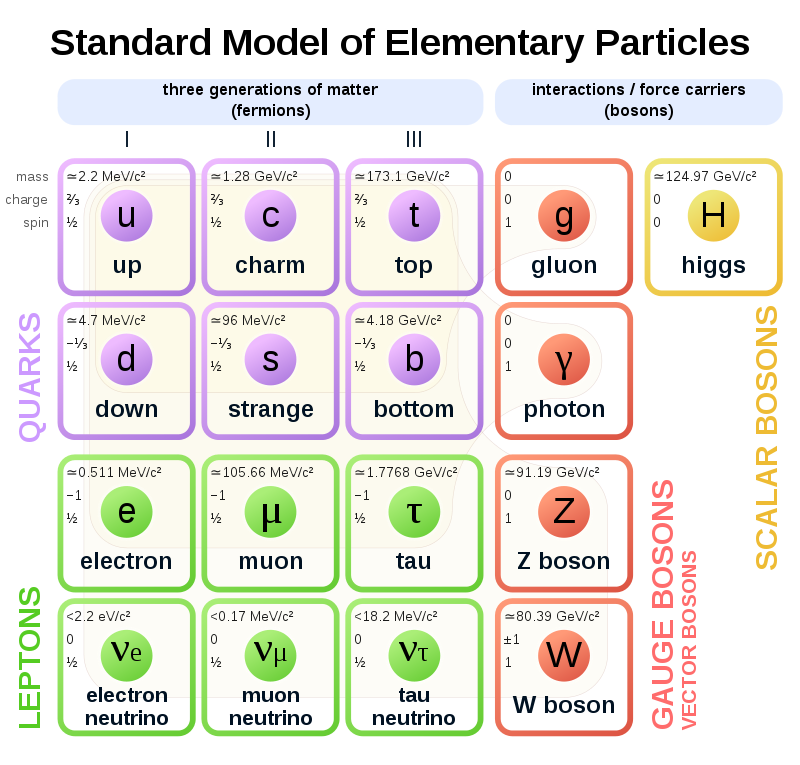
\includegraphics[width=0.65\linewidth]{introParticelle/ModelloStandard.png}
        \caption{Rappresentazione del Modello Standard}
        \label{fig:ModelloStandard}
    \end{figure}
    
Nella parte sinistra della figura \ref{fig:ModelloStandard} si trovano i \textit{fermioni} divisi tra quark e leptoni. Sono divisi in tre generazioni ordinate in base a valori di massa crescente. I quark sono contraddistinti dal sapore (ad esempio: top, down, charm, strange e bottom) e non possono esistere mai da soli ma formano solitamente barioni (3 quark) o mesoni (coppie di un quark e un anti-quark). Nella parte destra della figura \ref{fig:ModelloStandard} si trovano i \textit{bosoni} divisi tra i bosoni di Gauge, che sono i mediatori delle forze fondamentali previste dal Modello Standard e il bosone di Higgs, che è l'unico bosone scalare (di spin 0) identificato per la prima volta nel 2012 al Cern.

 
 
\section{I mesoni pesanti nello studio del QGP}
Il QGP è uno stato della materia in cui i quark e i gluoni non sono confinati negli adroni. Ad ALICE si vuole studiare questo stato della materia, ma ciò non può essere fatto attraverso osservazioni dirette. Gli adroni formati da quark pesanti (come il charm e lo strange) sono un buon mezzo per studiare il QGP formatosi dalla collisione di ioni pesanti. Questo perchè i quark piú pesanti si formano in tempi scala piccoli ($\leq 0.1 fm/c \simeq 0.3 10^{-24}$s) rispetto ai tempi di formazione del QGP ($\simeq 0.3 - 1.5 fm/c \simeq 10^{-24} - 0.5 10^{-23}$s). I quark pesanti preservano la loro identit\`a mentre attraversano il QGP e adronizzano poi formando adroni che possono essere osservati dai rivelatori di ALICE. I mesoni D sono formati da due quark, un charm e un down e sono pertanto adatti allo studio del QGP. 
\\Il QGP si forma in seguito a collisioni di ioni pesanti, mentre in questa tesi si \`e studiata la produzione del mesone $D^{*+}$ da collisioni di fasci di protoni. I dati sui mesoni D derivanti da collisioni pp vengono utilizzati come riferimento da confrontare poi con i dati derivanti da collisioni di ioni pesanti come Pb-Pb. 

\section{Il mesone $D^{*+}$} \label{mesoneD}
Il mesone $D^{*+}$ è formato da un quark charm $c$ e un anti-quark down $\overline{d}$ ed ha momento angolare totale 1. Il mesone $D^{*+}$ ha una massa di ($2010.26 \pm 0.05$) $MeV/c^2$ e vita media $ \tau = (7.89 \pm 0.11) {10^{-21}}$s \cite{PDG}. Il decadimento studiato in questa tesi \`e:  $D^{*+} \rightarrow D^0 + \pi^+ $ (decadimento forte) ed ha un branching ratio BR = $67.7$ $\%$. Studiando la cinematica di questo decadimento si pu\`o caloclare il Q-valore:
    \begin{equation}
        Q = m_{D^{*+}} - (m_{D^{0}} + m_{\pi_{soft}}) = 5.85 MeV/c^2
    \end{equation}
Se ne deduce che, nel caso in cui la $D^{*+}$ decada da ferma, il pione ha un impulso di $39 MeV/c$, per questo viene chiamato $\pi_{soft}$. % controllare valore impulso soft pi
La $D^0$ ha massa $ (1864.83 \pm 0.05) $ $MeV/c^2$, decade per decadimento debole $D^0 \rightarrow K^- \pi^+$ con un BR = $3.89$ $\%$ ed ha una vita media di $(410.1 \pm 1.5 ) 10^{-15} s $ \cite{PDG}.
\\La figura \ref{fig:decadimentoD} rappresenta la topologia del decadimento del mesone $D^{*+}$. 

    \begin{figure}[htbp]
        \centering
        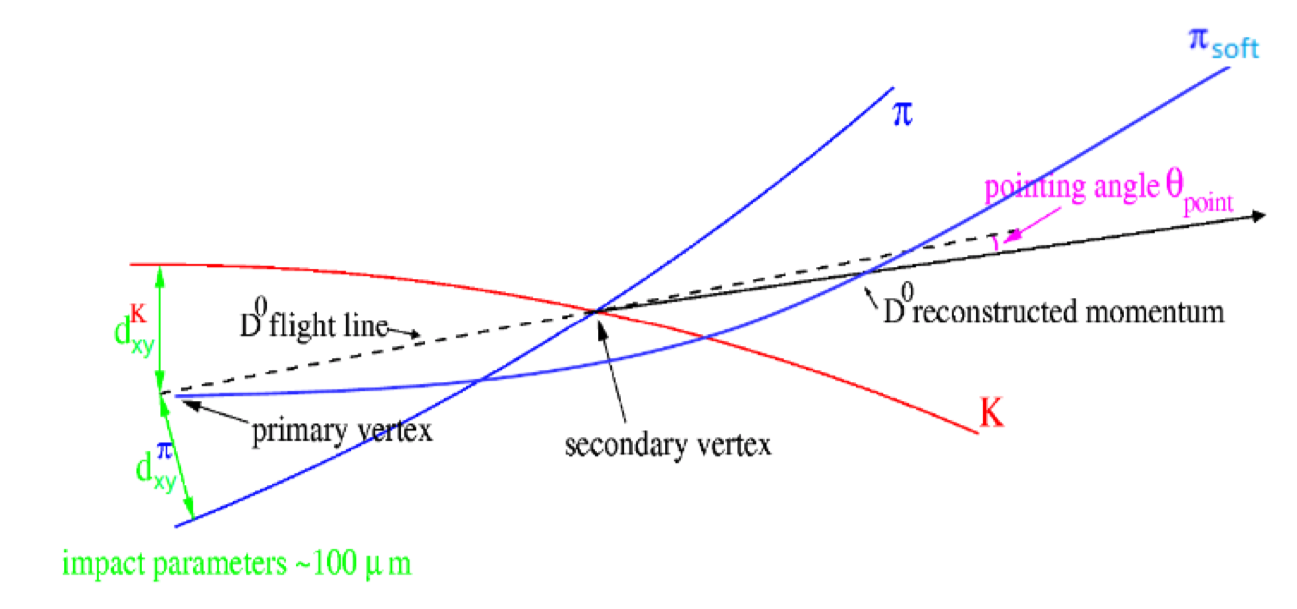
\includegraphics[width=0.9\linewidth]{introParticelle/DecadimentoDStar.png}
        \caption{ Schema del decadimento del mesone $D^{*+}$}
        \label{fig:decadimentoD}
    \end{figure}
In figura \ref{fig:decadimentoD} il punto di decadimento della $D^{*+}$ coincide con il vertice primario, ovvero il punto in cui avviene la collisione. Questo accade poich\`e i tempi che caratterizzano il decadimento forte della $D^{*+}$ non sono sufficienti per distinguere i due punti. Il punto di decadimento della $D^0$ (che decade debole) \`e, invece, distinguibile e viene chiamata vertice secondario.
\\Per identificare il mesone $D^{*+}$ inizialmente si ricostruisce la $D^0$ considerando tutte le possibili combinazioni di due tracce di segno oppostoe se ne calcola la massa invariante , che \`e definita come 
    \begin{equation}
        s = {E^2}_{TOT} - {p^2}_{TOT}
    \end{equation}
Nel caso della $D^0$ la massa invariante \`e  
    \begin{equation}
        s = ({E_{\pi^+}+E_{K^-}})^2 - ({p_{\pi^+}+p_{K^-}})^2
    \end{equation}
Quindi si aggiunge la traccia del $\pi_{soft}$ e si calcola la massa invariante della $D^{*+}$
    \begin{equation}
        s = ({E_{\pi^+}+E_{D^0}})^2 - ({p_{\pi^+}+p_{D^0}})^2
    \end{equation}
Si considera la distribuzione della differenza della massa invariante 
  \begin{equation}
       \Delta M = M (K^- \pi^+ \pi^+) - M(K^- \pi^+)
    \end{equation}
dove $ M (K^- \pi^+ \pi^+)$ \`e la massa ricostruita della $D^{*+}$ e 
$ M(K^- \pi^+)$ la massa ricostruita della $D^{0}$.
\\Per ridurre il fondo combinatoriale, derivante dalla combinazione di tracce non relative alle candidate $D^{*+}$, si fa una selezione in base alle distribuzione di alcune variabili topologiche del decadimento della $D^{*+}$. Le variabili topologiche riportate in figura \ref{fig:decadimentoD} sono:
    \begin{itemize}
        \item la lunghezza di decadimento della $D^0$, ovvero la distanza tra il vertice primario e secondario
        \item i parametri d'impatto del kaone e del pione (in figura \ref{fig:decadimentoD} indicati come ${d^K}_{XY}$ e ${d^\pi}_{XY}$ rispettivamente per kaone e pione) sono la distanza minima tra la traiettoria di kaone o pione e il vertice primario
        \item l'angolo di pointing, indicato come $\theta_{point}$, \`e l'angolo tra la retta congiungente il PV e il SV e la direzione del $p_T$ della $D^{*+}$
        \item l'angolo di decadimento, che \`e l'angolo tra il vettore impulso del mesone $D^0$ e il vettore impulso del $\pi^+$ nel sistema di riferimento della $D^0$
        \item la distanza di minimo approccio (DCA) \`e la distanza minima tra le traiettorie del $K^-$ e del $\pi^+$ nel piano perpendicolare alla direzione del fascio
    \end{itemize}{}

Nell'analisi standard di ALICE, per la selezione delle $D^{*+}$, vengono scelte manualmente le selezioni da applicare sulle variabili topologiche. 






